%!TEX root = ../dissertation.tex
\begin{savequote}[75mm]
Language is a process of free creation; its laws and principles are fixed, but the manner in which the principles of generation are used is free and infinitely varied.
\qauthor{Noam Chomsky}
\end{savequote}

\chapter{Dynamic Multimodal Network}

\newthought{On this chapter, a new model to handle language and vision features to define a segmentation mask is proposed}, by merging previous ideas and insights (as they were described on Chapter \ref{chap:previous_work}) with state-of-the art models in both visual and language recognition tasks. This model shall take the name of Dynamic Multimodal Network (DMN), as it not only processes language and visual information in a recurrent fashion \cite{li2017cvpr} (Multimodal Network) by taking visual and language information as a concatenated entity \cite{hu2016segmentation}, but it also generates and applies a set of dynamic filters based on the language representation to the visual one at each time step, inspired on \cite{liu2017segmentation}. Additionally, a new sampling module is proposed, based on the effectiveness of skip connections \cite{DBLP:journals/corr/RonnebergerFB15} to refine and produce segmentation masks that fit each object contour accordingly.


\begin{figure}
\centering
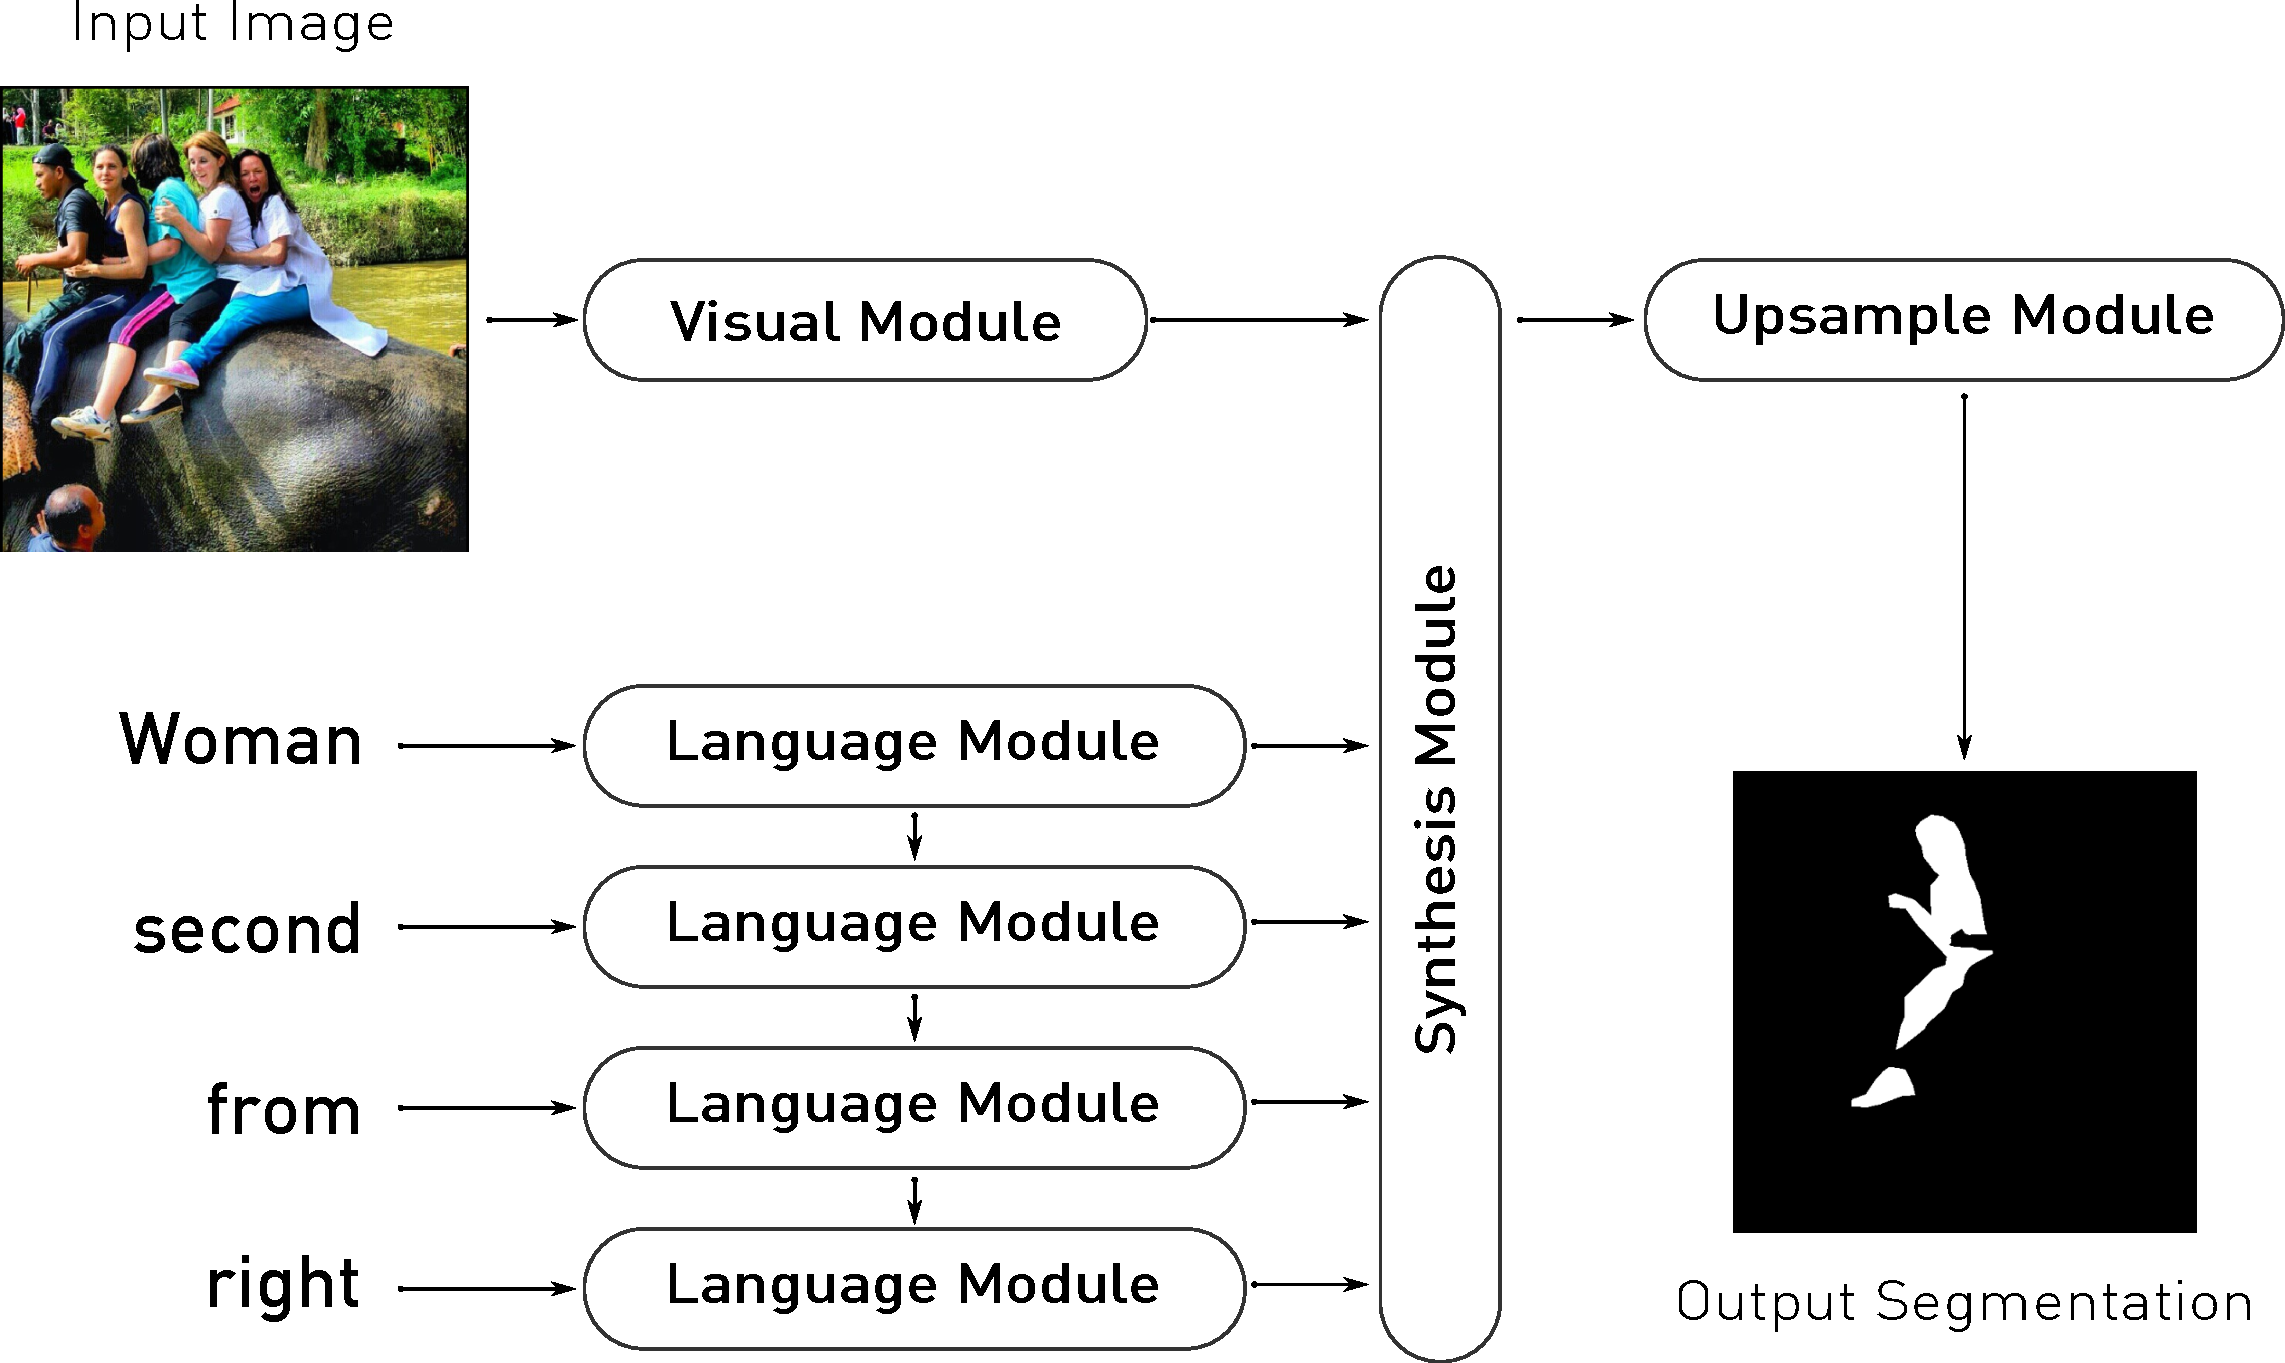
\includegraphics[width=\textwidth]{./figures/Model_Overview.pdf}
\caption{Dynamic Multimodal Network general overview consisting of a Visual Module, a Language Module, a Synthetic Module and a Upsampling Module}
\label{Fig:Overall}
\end{figure}

As shown on Figure~\ref{Fig:Overall} The DMN consists of four modules, one per each subtask proposed. The first two modules (Visual and Language modules\footnote{VM and LM, respectively}) handle each input to the model separately, extracting and modelling a representation for each modal input. Then, the Synthetic Module (SM) takes both representations and combines them to generate a low resolution segmentation mask. Finally, the Upsampling Module (UM), produces a higher resolution mask based on the output of the previous module.

The model consists of a Fully Convolutional Network (FCN) model for the VM and two Recurrent Neural Networks for the LM and the SM. The UM consists of a sequence of Convolution and Bilinear Upsampling layers that produce a $(H, W)$ mask from a low resolutuion mask of size $\left(\frac{H}{32}, \frac{W}{32}\right)$. On sections \ref{section:vm} - \ref{section:um} each module is presented and described on a more detailed way.

\section{Visual Module (VM)}
\label{section:vm}

\begin{figure}
\centering
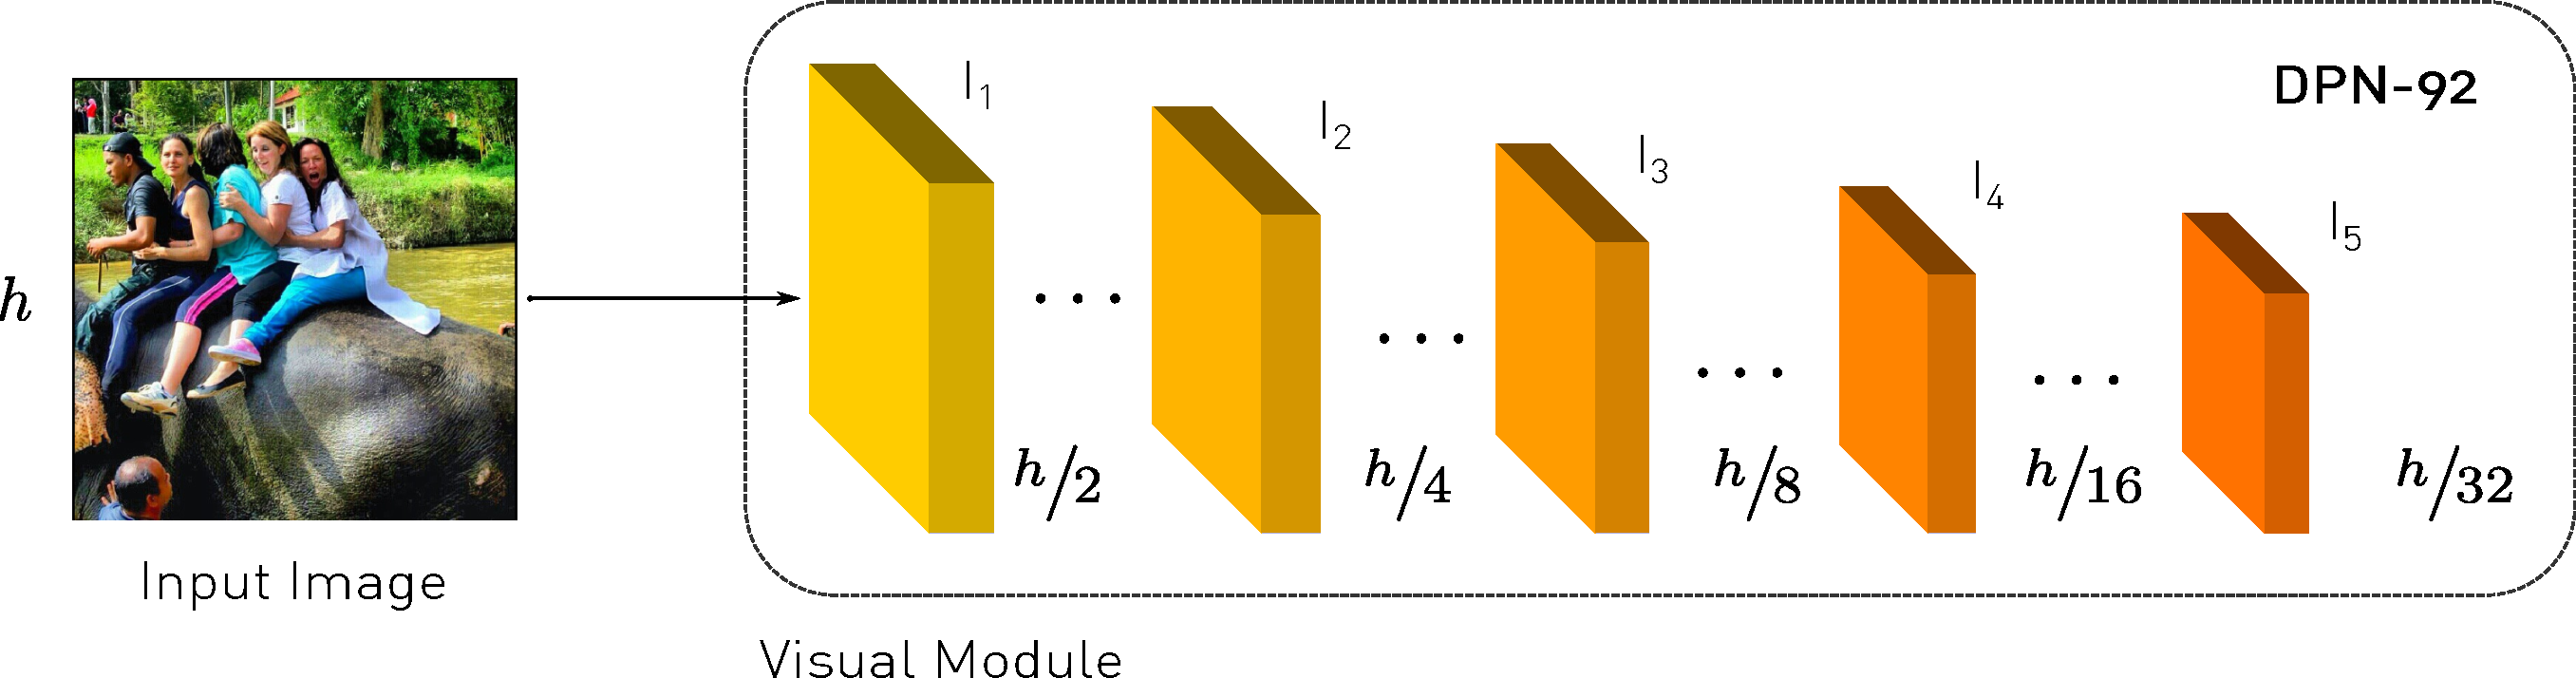
\includegraphics[width=\textwidth]{./figures/Visual_Module.pdf}
\caption{Visual Module overview}
\label{Fig:VM}
\end{figure}


The Visual Module (Figure~\ref{Fig:VM}) extracts features from an input image using a Fully Convolutional Network (FCN), these kind of models are able to take as input images of different dimensions, and therefore enables the DMN to process images of any arbitrary size. As the model depends on the multiscale features produced by the FCN, it is expected that as the FCN model improves its performance, as the visual features extracted from an input image should be more descriptive. Given this idea, the DMN experiments were based on the Dual Path Network-92 (DPN-92) \cite{DBLP:journals/corr/ChenLXJYF17}, due to its competitive results in various tasks and its parameter size efficiency.

Given an input image $I$, the VM produces a 5-tuple $\{I_1, I_2, I_3, I_4, I_5\}$, where each $I_k$ corresponds to the DPN-92 features of size $\frac{H}{2^k}$. As each map contains different resolution level features, it is expected that the encoded information helps to produce better segmentation masks, by including them on the last module.


\section{Language Module (LM)}
\begin{figure}
\centering
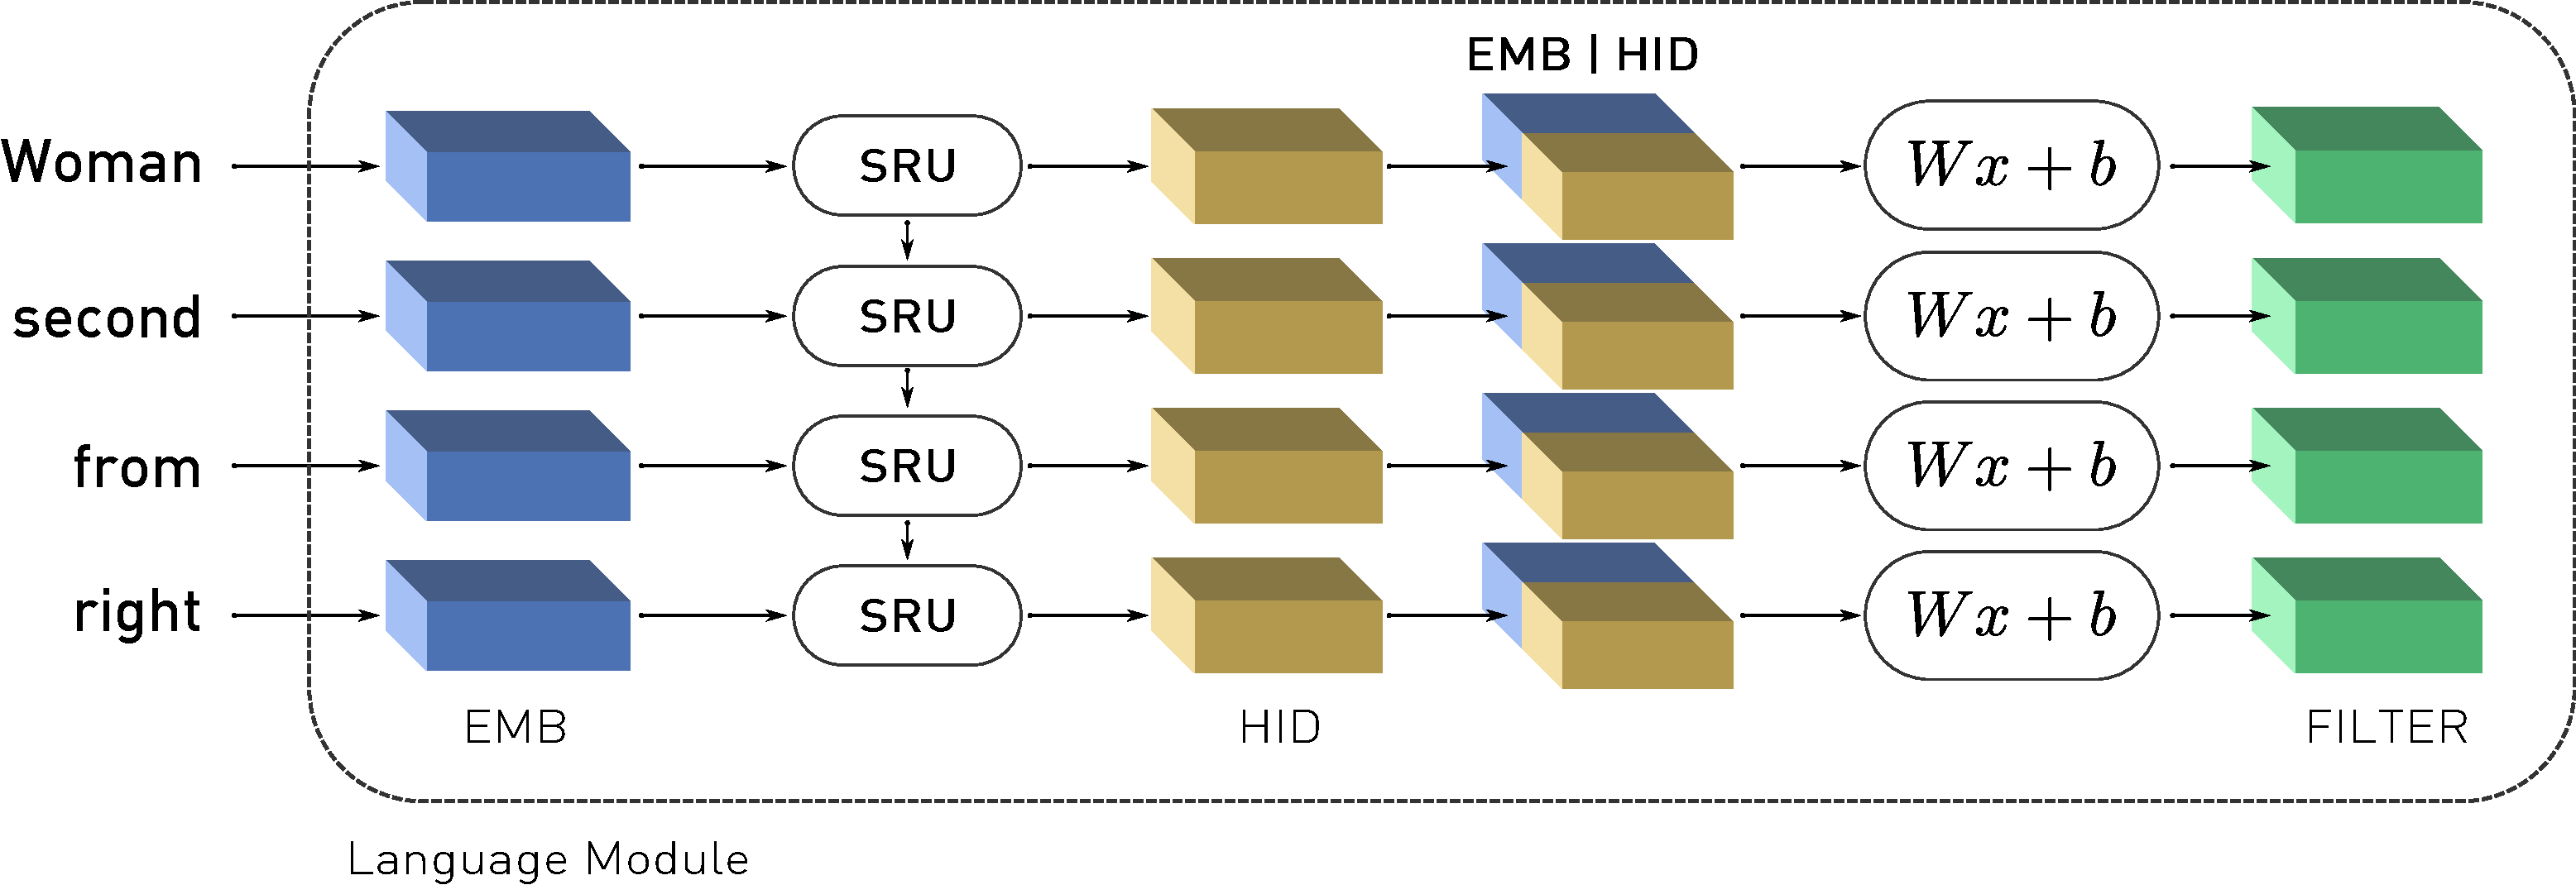
\includegraphics[width=\textwidth]{./figures/Language_Module.pdf}
\caption{Language Module overview}
\label{Fig:LM}
\end{figure}

This module extracts and models language features from an input query and outputs a sequential representation for each word, including a word embedding (WE/EMB), a temporal sequence representation (Hidden state) and a dynamic visual filter based on the previous two representations. As shown on Figure~\ref{Fig:LM}, the model employs a WE representation trained from scratch, such that each dataset vocabulary (Which may contain several thousands of words) can be described on a lower dimensional space such that near language concepts are also near on the resulting embedding.

To model the overall embedding sequence and produce a sequence of hidden states (HID) that represent each word given the previous ones, the DMN employs a Recurrent Neural Network (RNN) model, and more specifically it is based on Simple Recurrent Units (SRU) \cite{DBLP:journals/corr/abs-1709-02755}, which reduce the overall training time with respect to classic RNN models, based on Gated Recurrent Unit (GRU) and Long Short Term Memory (LSTM) units, while achieving better results than the aforementioned models.

From the sequential outputs of the RNN and their corresponding embeddings, the LM produces a set of "language-based visual filters" (FILTER) using a linear layer of $F$ dimensions. Formally, the Language Module can defined as \eqref{eq:lm}, where $\left\{w_i\right\}_{t=0}^{T}$ refers to a sequence of words of length $T$, $e_i$ to their corresponding WE, $h_t$ to the hidden states and $f_{tj}$ to each of the $F$ filters computed per each word.
\setlength{\abovedisplayskip}{0pt}
\setlength{\belowdisplayskip}{0pt}
\begin{alignat}{2}
\left(\left\{h_t\right\}_{t=0}^{T}, \left\{e_t\right\}_{t=0}^{T}, \left\{f_{tj}\right\}_{t=0}^{T} \right) &= LM\left(\left\{w_i\right\}_{t=0}^{T}\right) \quad j \in [0, F) \label{eq:lm}
\end{alignat}


\section{Synthesis Module (SM)}
\begin{figure}
\centering
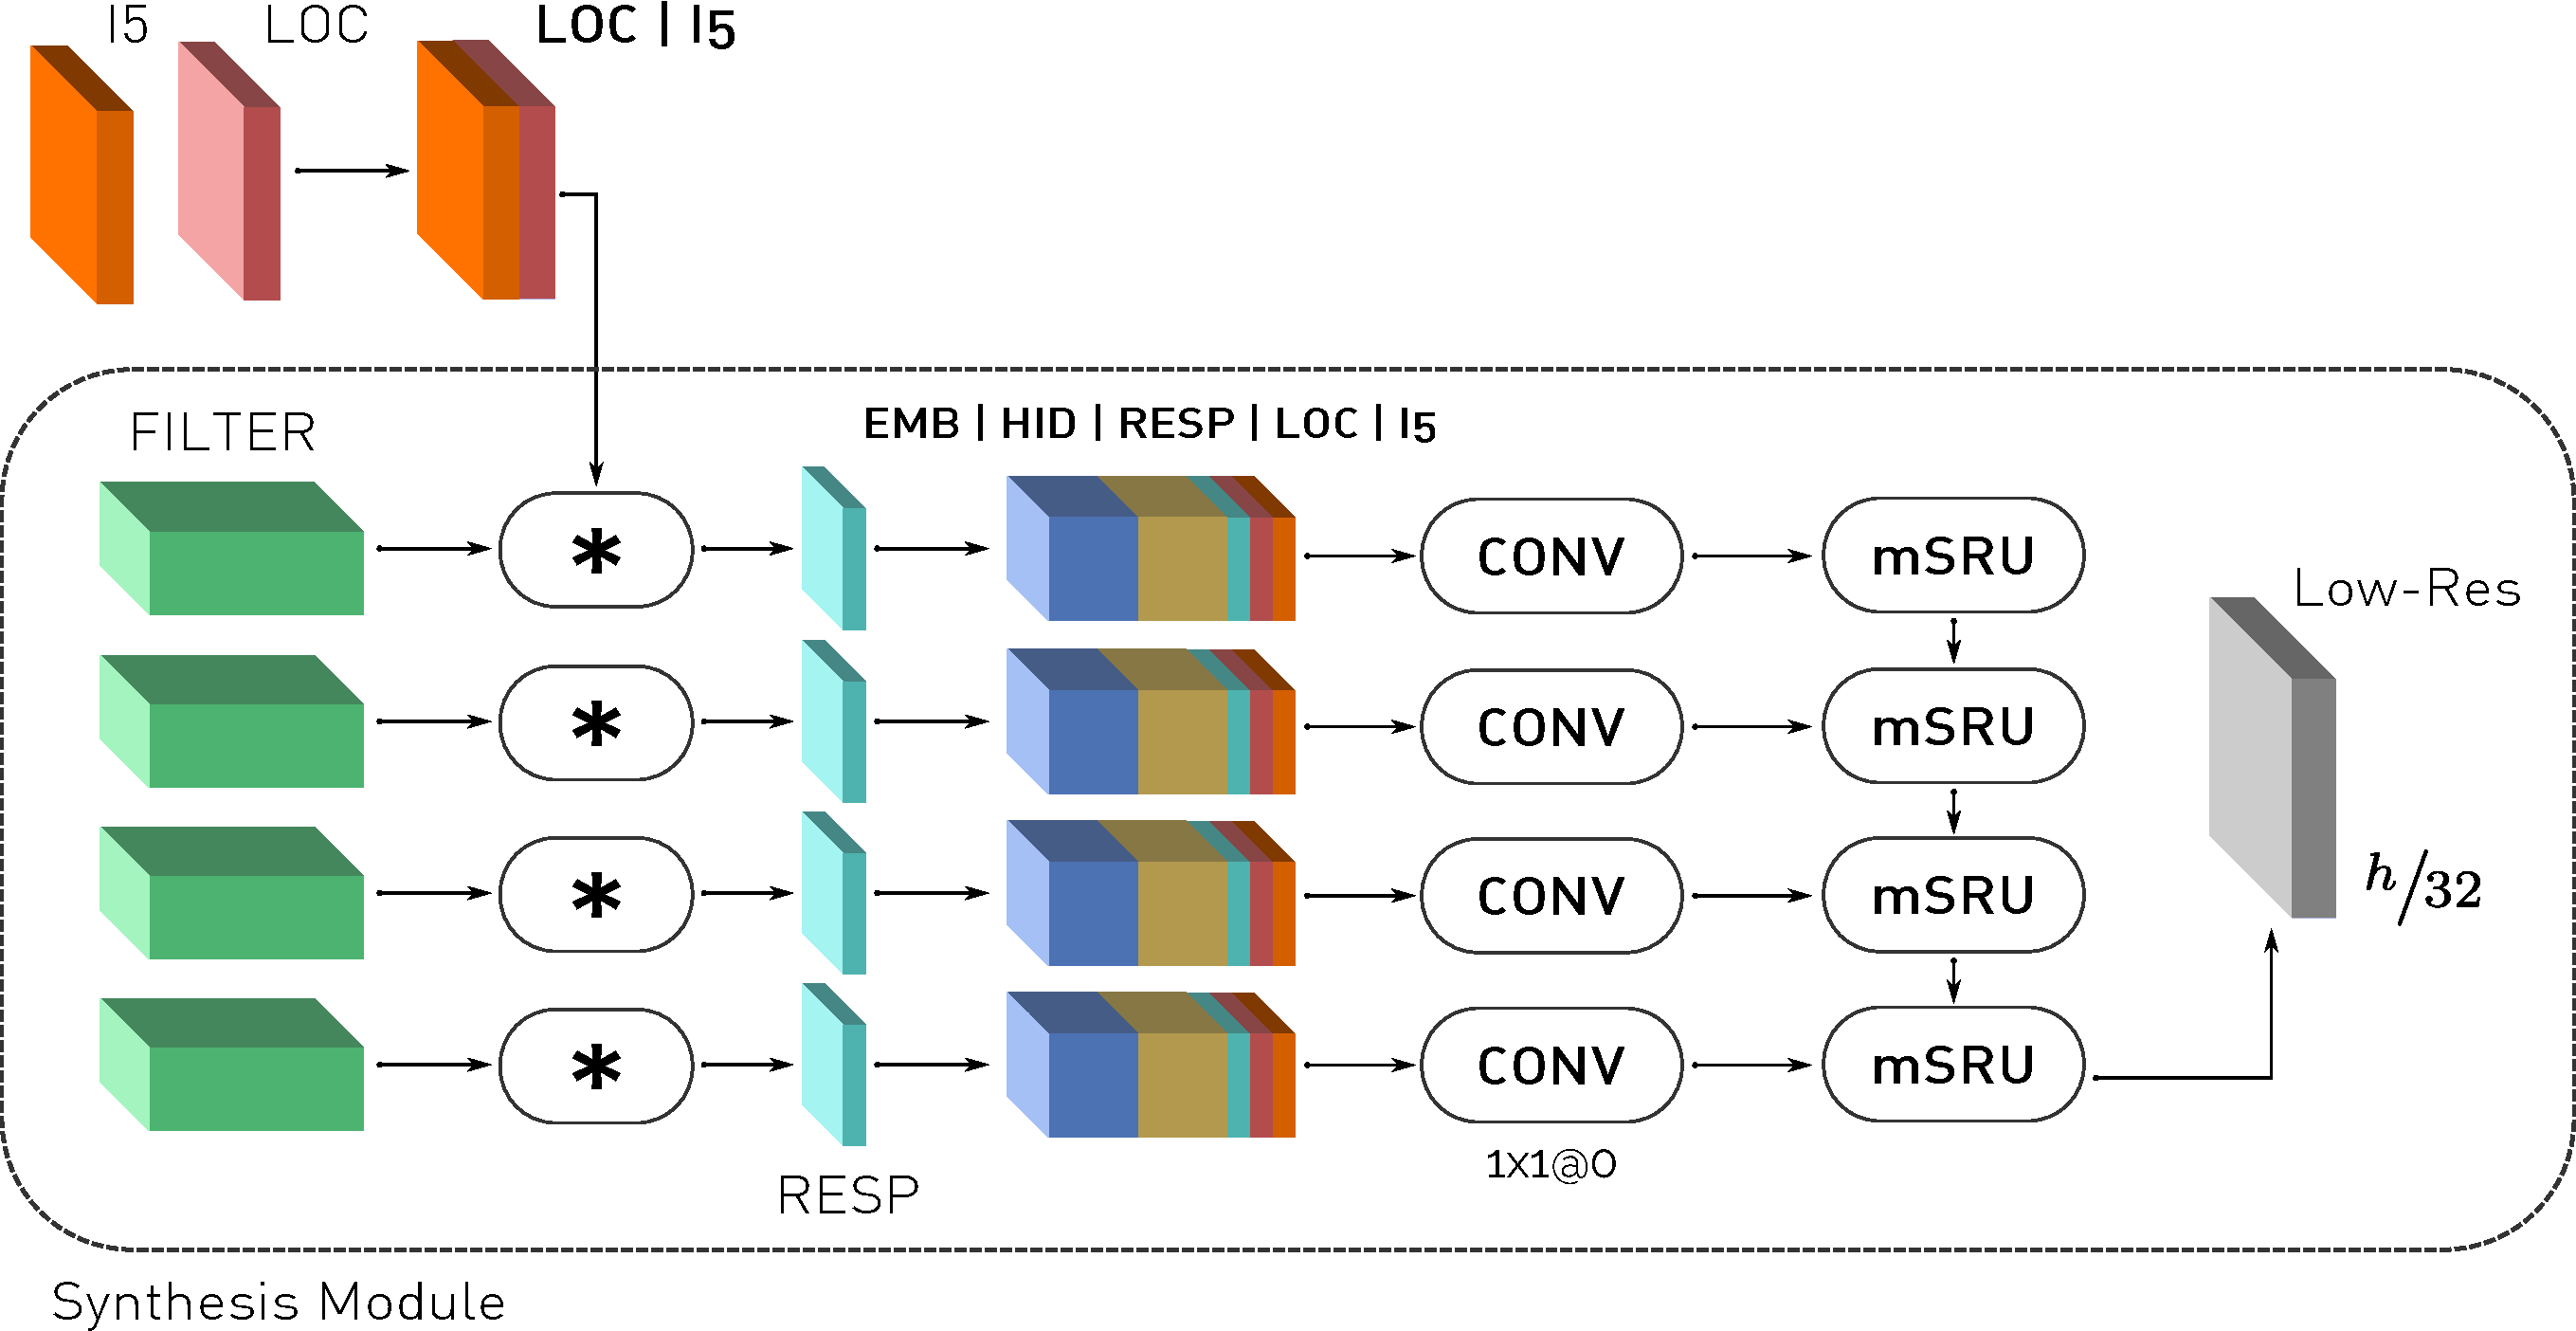
\includegraphics[width=0.9\columnwidth]{./figures/Syn_Module.pdf}
\caption{Synthesis Module overview}
\label{Fig:SM}
\end{figure}

The Synthesis Module represents the core module of the DMN, as it merges both visual and language information in a sequential manner. As it can be seen on Figure~\ref{Fig:SM}, for each time $t$ the model takes into account all the previous information and concatenates them into the spatial channels of the low resolution filter response $I_5$ produced by the VM, which in turn are also concatenated with a set of static image coordinate maps, which improve the localisation outputs of the network. With respect to the language filters produced by the LM, they are applied to the visual response and also to the localisation maps via convolution and the overall response map is also appended to the multimodal representation as an additional channel.

The DMN uses a mSRU (Multimodal SRU) that takes as input each one of the multimodal representation at each time (after applying a convolution layer of kernel size $1 \times 1$), and by taking the last $\left(\frac{H}{32}, \frac{W}{32}\right)$ values of the last hidden state, it produces a low resolution segmentation mask (LR). By processing the mulimodal information in a sequential way, the SM exploits the sequential nature of language, which also applies to the combined visual task.


\section{Upsampling Module (UM)}
\label{section:um}
\begin{figure}[!h]
\centering
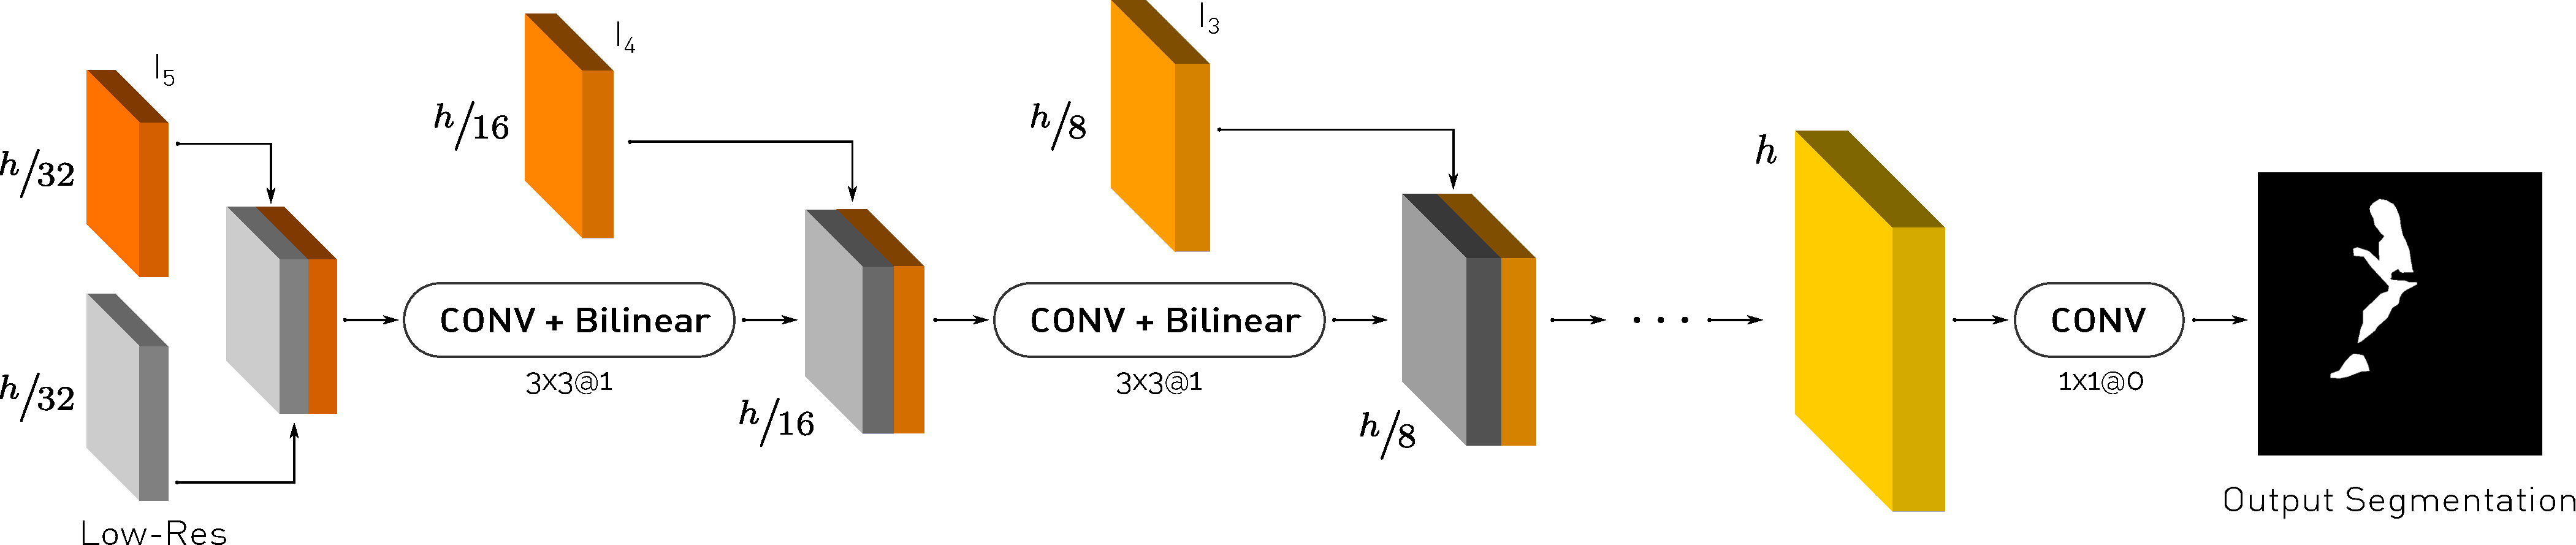
\includegraphics[width=\columnwidth]{./figures/Up_Module.pdf}
\caption{Upsampling Module overview}
\label{Fig:UM}
\end{figure}
The last component of the DMN architecture corresponds to the Upsampling module, and as its name implies, this modules does take a low resolution segmentation mask input to produce a high resolution one that has the same dimensions of the input image.

To perform such operation (Figure~\ref{Fig:UM}), the UM is based on incremental size upsampling operations that take advantage of the visual multi resolution maps gathered by the Visual Module, therefore, on each upsampling phase, each partial upsampling map $U_k$ is concatenated alongside its corresponding visual map $I_k$, to produce an output map $U_{k+1}$ of size $\frac{H}{2^{k+1}}$. This implies a total number of 5 upsampling submodules in the UM architecture.

To prevent artifacts on the resulting segmentation mask introduced by using transposed convolutions\footnote{Also known as \textit{''deconvolutions''}} and also to produce smooth and refined segmentation outputs, each upsampling submodule is composed of a Convolution layer and a bilinear upsampling layer. 